In this section, we provide two ways to construct an order-4 apeirogonal tiling of the hyperbolic plane.

\subsection{A construction based on order-4 Cayley tree}\label{sec:tree}

We define a domain $D$ in the Euclidean plane as follows. Let $D$ be the union of the following regions:

\begin{figure}
    \centering
    
\includegraphics[width=0.2\textwidth]{images/cayley-tree-4-border-2.pdf}
    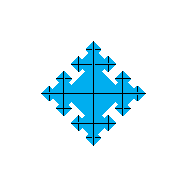
\includegraphics[width=0.2\textwidth]{images/cayley-tree-4-border-3.pdf}
    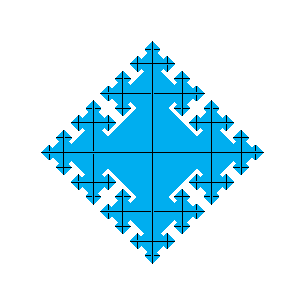
\includegraphics[width=0.2\textwidth]{images/cayley-tree-4-border-4.pdf}
    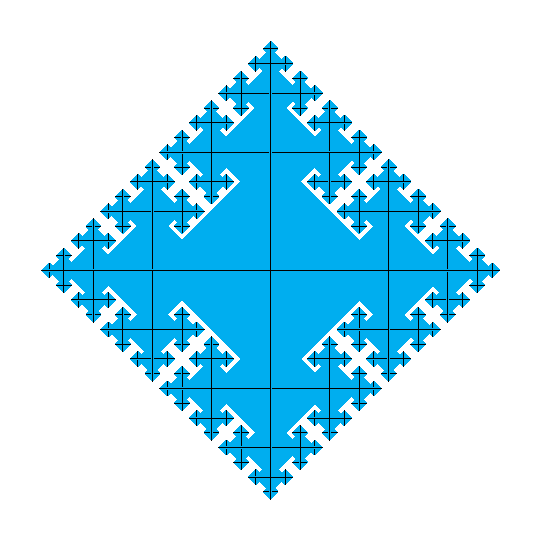
\includegraphics[width=0.2\textwidth]{images/cayley-tree-4-border-5.pdf}
    \caption{construction step 2, 3, 4, and 5 of the domain $D$}
\end{figure}

\subsection{Construction of order-4 apeirogonal tiling}\label{sec:tiling}

\subsection{Coloring and compatible coordinate}\label{sec:coloring}
